Before analysing the results of the systematic literature review, we present the protocol of this review and discuss the strengths and weaknesses of this work. The methodology of the systematic review is largely based on \cite{weidt_systematic_2016} and complemented by the work of \cite{xiao_guidance_2017,petticrew_systematic_2008,snyder_literature_2019,denyer_producing_2009}. We used the eleven steps presented in \cite{weidt_systematic_2016} to structure our systematic review.

\subsection{Review Protocol}

The review protocol of this work is structured according to \cite{weidt_systematic_2016} and will be presented in this subsection. The protocol is structured according to \cite{weidt_systematic_2016} and should allow the reader to evaluate the objectivity and quality of the final results (\cite{page_prisma_2021}). The review protocol was iterative developed, and the final result is presented.


\subsubsection{Defining the main research questions of the literature review}

Based on the need for an updated review of the research field concerning web survey participation with smartphones, we developed three research questions:

\begin{itemize}
   \item \textbf{Research Question 1}: Which characteristics of the use of smartphones in web surveys are researched on, and what are research gaps in the field? 
   \item \textbf{Research Question 2}: Which dimension comparing the data quality between smartphones and PC in web surveys are investigated, and which factors lack qualitative research?
   \item \textbf{Research Question 3}: Which elements of online survey design are investigated for adjustments to the use of smartphones, and which aspects are missing in current research?
\end{itemize}

\subsubsection{Defining keywords}
\label{subsubsec: Defining search string}

After a first literature search and multiple iterations, we identified the following search string for our literature search: \\

\begin{quote}
    (“mobile” OR “phone” OR “tablet” OR “device”) \\

    AND ("web" OR "online" OR "digital" OR "browser ")  \\
    
    AND ("survey" OR "question*" OR "panel" OR "poll")  \\
    
    NOT ("bank*" OR "payment" OR "e-commerce" OR "health" OR "shop*" OR "library" OR "education" OR "sex*" OR "dating" OR "tourism" OR "travel" OR "social network" OR "social media" OR "internet of things" OR "iot" OR "advertise*")\\
\end{quote}

We identified the final combination of terms based on the precision and recall of the search terms combined with advanced search settings for retrieving relevant entries while working with the databases. The first three lines should ensure that we find all relevant articles (improve recall), while the last line should ensure that we do not find too many non-relevant records (improve precision).


\subsubsection{Defining search engines}
\label{subsubsec: Defining search engines}

We selected the search databases based on recommendations of the library of the University of Mannheim and the evaluations in the articles of \cite{pascoe_systematic_2021, papaioannou_literature_2010, gusenbauer_which_2020}. We complemented the list with the database of the publisher of influential Journals in the research area. We excluded databases and articles where we had no free access as a student of the University of Mannheim. If a search engine had multiple databases included, we mark the databases selected. The resulting final list comprised the following six databases:

\begin{itemize}
    \item  Web of Science
    \item ProQuest
    \begin{itemize}
        \item Applied Social Sciences Index \& Abstracts (ASSIA)
        \item Business Market Research Collection
        \item Sociological Abstracts
        \item Worldwide Political Science Abstracts
    \end{itemize}
    \item EBSCO
    \begin{itemize}
        \item APA PsycArticles
        \item APA PsycInfo
        \item PSYNDEX Literature with PSYNDEX Test
        \item Communication \& Mass Media Complete
    \end{itemize}
    \item Sage Journal
    \item Oxford Publisher
    \item Tanford Publishing
\end{itemize}

\subsubsection{Search string execution}

Based on the search string in \ref{subsubsec: Defining search string} we conducted the search in the databases mentioned in \ref{subsubsec: Defining search engines} on the 20.12.2021. Additional settings in the search engine that were used when applicable are presented in table \ref{tab: search settings}. The search was conducted by searching in the title, abstract, and keywords. If a combined search of these fields was not possible, we searched only in the abstract.

\begin{table}
	\centering
	\begin{tabular}{ll}
		\toprule
		Settings & Values \\
		\midrule
		Time Horizon & Publications from year 2008 to 2021 \\ 
		Literature Type & Research articles published in peer-reviewed \\
		& proceedings and journals \\
		Research Field & Social Science, Political Science, Business, Economics, \\
		& Computer Science, Psychology, Communication \\
		Language & English \\
		\bottomrule 
	\end{tabular}
	\label{tab: search settings}
	\caption{Additional settings for the search engines of the bibliographic databases}
\end{table} 

\subsubsection{Download and store search results}

The bibliographic details of the search results were downloaded as .ris files by offered download functions or scraped directly from the site with the bibliographic program Mendeley. The resulting files were saved and managed in Mendeley and Zotero's bibliographic programs. We found 2787 records in the search, which resulted in 1580 non duplicate entries.

\subsubsection{Define inclusion and exclusion criteria}
\label{subsec: Inclusion and Exclusion Criteria}

For the final selection of relevant articles for the systematic literature review, we defined a set of inclusion and exclusion criteria. These criteria are the foundation to determine relevant research articles in the selection stage.

\paragraph{Inclusion Criteria}
\begin{itemize}
    \item Research articles that focus on mobile web surveys
    \item Research articles that explicitly state the role of smartphones in mobile web surveys
    \item Research articles that are in English
    \item Research articles that were published between 2008 and 2021
    \item Research articles that are published in a peer-reviewed journal
    \item Research articles that are published in a peer-reviewed conference proceeding
\end{itemize}

\paragraph{Exclusion Criteria}
\begin{itemize}
    \item Research articles that do not differentiate the effects of different mobile devices like tablets and smartphones
    \item Research articles that use mobile devices only under the supervision of an interviewer
    \item Research articles that include mobile devices in web surveys without specifically analysing their impact
    \item Research articles on mobile forms in general
    \item Research articles focusing on mobile web tests or assessments
    \item Research articles about passive data collection with the smartphone
    \item Research articles that only focus on a small, unrepresentative group in medical trials
    \item Research articles that present specifically developed software
\end{itemize}

\subsubsection{Selection of papers - First and Second stage}

We screened the results of the literature search by title, abstract, and full text based on the in section \ref{subsec: Inclusion and Exclusion Criteria} defined inclusion and exclusion criteria. The title screening resulted in 147 selected records, which were reduced to 104 articles in the abstract screening. We found 12 additional articles in a back and forward citation search, resulting in 116 articles for the full-text screening. After the last screening stage, we identified the final sample of 86 articles. The entire process of the selection of the records can be retraced in the Prisma statement ( \ref{fig: Prisma Statement}) of this review.

\begin{figure}
    \centering
    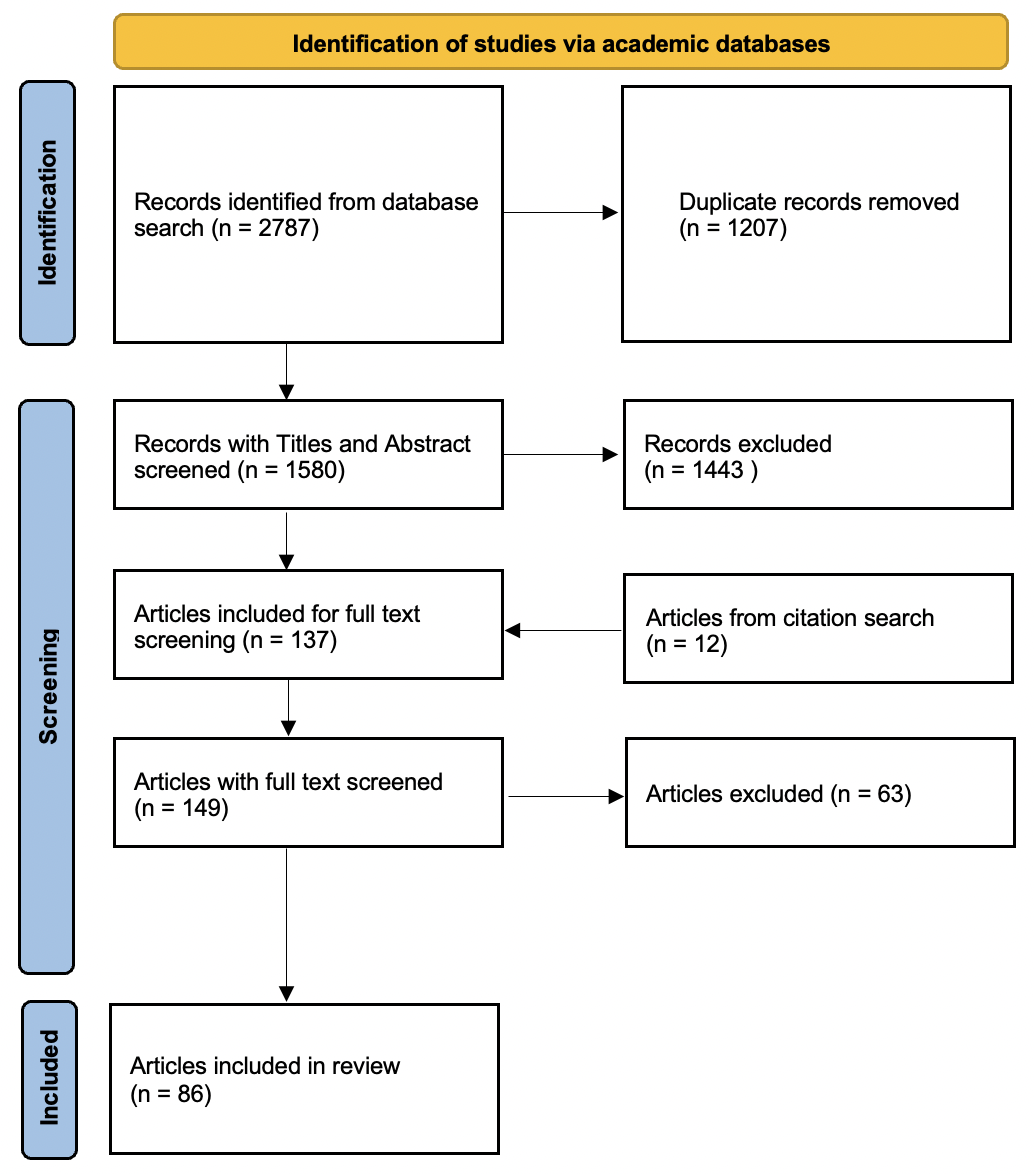
\includegraphics[width=\textwidth]{reports/figures/Prisma Statement.png}
    \caption{Prisma Statment for the systematic literature review in accordance with \cite{page_prisma_2021}}
    \label{fig: Prisma Statement}
\end{figure}

\subsubsection{Extraction of answers related to research questions}

After the selection, the information for analysing the research questions was extracted by a single coder. The information was saved in a spreadsheet that was used for further analysis. The interested researcher can refer to all results of the review in the accompanying GitHub Repository (\cite{langenbahn_smartphone_2021}).


\subsection{Discussion of procedure}

We critically discuss the procedure of the systematic literature review in this section to enable the reader to evaluate the objectivity and validity of the presented results. The article was written in postgraduate coursework by a single student. That is why we choose the guideline from \cite{weidt_systematic_2016} based on their feasibility for postgraduate students and the possibility to use the guidelines as a single reviewer. Other approaches and procedures as presented in \cite{xiao_guidance_2017,petticrew_systematic_2008,snyder_literature_2019,denyer_producing_2009} may be more appropriate for a more professional setup but were out of the scope of this coursework. 


\subsubsection{Analysis of bias in this work}

We will base our analysis for bias on \cite{durach_new_2017} which identifies the bias classes: sample bias, selection bias, within-study bias and expectancy bias.

The class of sample bias divides into retrieval and publication bias, which are both to a certain degree present in this work. Retrieval bias may occur in selecting databases, creating the search strings, and the search settings used. Our choice of databases was based on best practices promoted by the University of Mannheim library, and the results of \cite{pascoe_systematic_2021, papaioannou_literature_2010, gusenbauer_which_2020}. However, this selection was limited to the resources available to University of Mannheim students, which excluded access to search engines like SCOPUS and some articles hidden behind a paywall. This restriction will have led to a high probability of a retrieval bias. The search string and settings showed a high recall with only 12 added articles from forward and backward citation search. As we included all important Journals and a wide range of databases, it is not probable that we have missed whole clusters of research articles that we could not identify in the citation search. However, the search string has a very low precision, which has led to much ineffectual work, potentially inducing mistakes in the selection. Another possible retrieval and publication bias is that this review only used articles published in a peer-reviewed scientific medium. Our citation search has shown that there are many impactful scientific works presented at conferences like the AAPOR Annual Conference or the CASRO Online Research Conference in a presentation format or the editor reviewed Journal Survey Practice. An enhancement could include these publications and grey literature in their review to get a more comprehensive overview of the research field. However, this will induce much work in revising the quality of the publication, which was not feasible in this work.

Selection biases partition into inclusion and selector biases, where an inclusion bias is highly likely in this work and the selector biases relatively insignificant. An inclusion bias implies not adequately defined inclusion and exclusion criteria. This bias will most likely be present in this work as no research experts for mobile web surveys designed the criteria. The selector bias is not significant through the setup with only one person creating inclusion and exclusion rules and selecting the articles, not offering much potential for inconsistencies.

The within-study bias describes errors in extracting information from the selected articles. As only one person extracted information from the data, we cannot guarantee the extraction quality by measurement like the inter-annotator agreement or similar. This setup can lead to an underestimated within-study bias for this work.

The expectancy bias is negligible in this work. The author of this work does not have any prior professional knowledge about mobile web surveys and personal interests that could lead to any preconceptions.

\subsubsection{Future research}
Finally, we want to discuss how another researcher could advance this review on the level of a scientific publication. We have already identified methodological weaknesses in the last section that need to be fixed. Additionally, we will shortly discuss the range of topics in this work. To avoid technical mistakes, the replication of this work would need at least one experienced researcher with expertise in mobile web surveys to use their domain knowledge and avoid the identified technical biases. Additionally, another researcher is required to increase the robustness of the selection and information extraction. With more resources, it would be possible to reduce the retrieval bias by including more search engines like SCOPUS and gaining access to paid articles. Further improvements could be the fine-tuning of the search string and the inclusion of the characteristics of different search engines. To further avoid publication bias, one could include qualified scientific literature not considered in this review. As this article is limited in its scope, we could not perform sophisticated meta-analyses and quantitative summaries but had to limit ourselves to an overview of the research field. In a following research project, one could concentrate on one dimension of smartphone web surveys. To summarise, we can state that the present work does not wholly fulfil all scientific standards but functions as a basis for further research work by reducing the workload and serving as quality control. 